\textbf{/F40/} \\
\textbf{Prozess:} Treffpunkt (Ort/Zeit) festlegen (Admin)\\
\textbf{Ziel:} Mitglieder erhalten definitive Angaben für den nächsten Termin\\
\textbf{Kategorie:} primär\\
\textbf{Vorbedingung:} feste Gruppe existiert, Mitglieder sind bestimmt, Administrator ist festgelegt\\
\textbf{Nachbedingung (Erfolg):} Alle Mitglieder können sehen, wann und wo (optional) das nächste Treffen stattfinden wird\\
\textbf{Nachbedingung (Fehlschlag):} Gruppenmitglied bekommt keine Einsicht zu den Daten des nächsten Treffens\\
\textbf{Akteure:} Gruppenadministrator\\
\textbf{Auslösendes Ereignis:} Ein neues Treffen ist in Planung\\
1.) Gruppenadministrator macht sich Gedanken, wann und wo das nächste Treffen der Gruppe stattfinden soll\\
2.) Er tippt auf den Namen der Gruppe und sieht die allgemeinen Informationen über die Gruppe (Namen, Mitglieder)\\
3.) Er tippt auf den Button "Ereignis erstellen"\\
4.) Er wird weitergeleitet zu einem neuen Fenster, in dem er aufgefordert wird Zeit und vorläufigen Treffpunkt des nächsten Treffens einzugeben\\
5.) nach Eingabe von mindestens einem der beiden Parameter, kann er das neue Treffen über einen Button "Treffen bestätigen" bestätigen\\
6.) nach Bestätigung des Treffens, wird ihm angezeigt\\
6.a) ob das Erstellen des neuen Treffens erfolgreich war
6.b) oder ob das Erstellen des neuen Treffens nicht erfolgreich war.
7.a) war das Erstellen des neuen Treffens erfolgreich, so wird er zurück geleitet auf die Gruppe und bekommt nun, wie alle Gruppenmitglieder die auf die Gruppe tippen, zusätzlich zu Namen und Mitglieder das neue Treffen angezeigt, das mit Zeit und Treffpunkt zu sehen ist\\
7.b) war das Erstellen des neuen Treffens nicht erfolgreich, so wird ihm in einem kleinen Fenster im Vordergrund angezeigt, welcher Fehler aufgetreten ist und er wird zur erneuten Eingabe aufgefordert. Durch drücken des Buttons "okay" wird das kleine Fenster geschlossen und er kommt zurück zu Punkt 4)\\ \\

\begin{figure} [H]
	\centering
	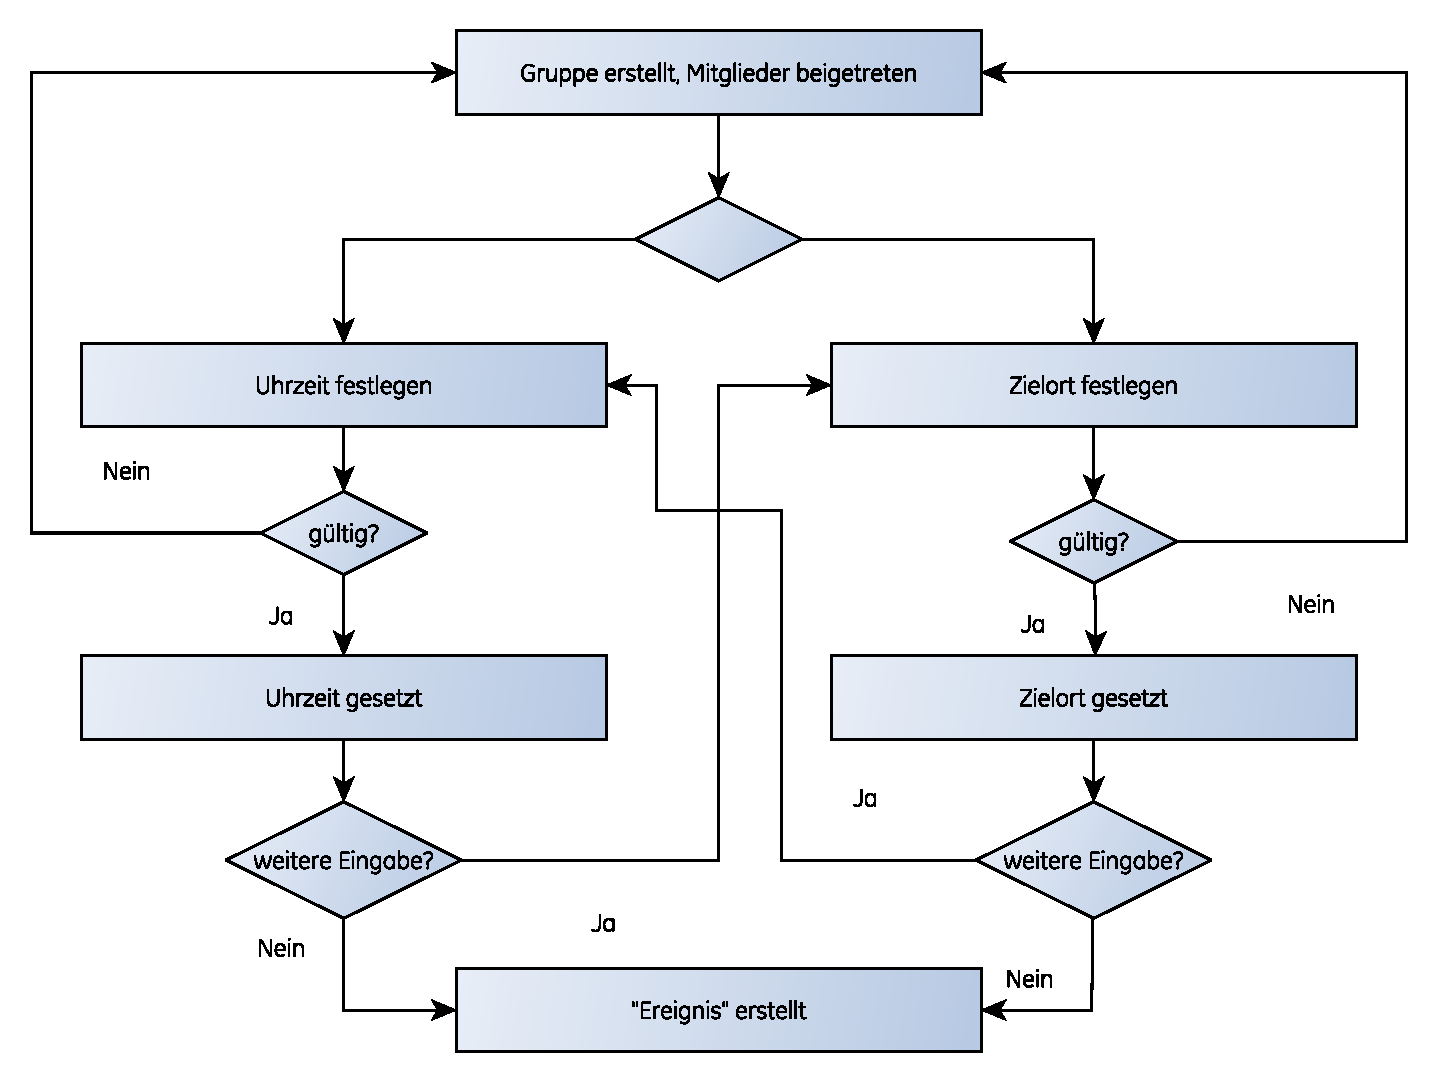
\includegraphics[scale=0.7]{./res/F40_ereignis_erstellen_flowgraph.pdf}
\end{figure}

